\documentclass[a4paper,12pt]{article}
\usepackage{fullpage}
\usepackage{amsmath}
\usepackage{graphicx}
\usepackage{subfig}
\usepackage{setspace}

\setlength{\parindent}{0pt} 

\begin{document}

\textbf{Graphene Basics} \\

The energy-momentum dispersion in graphene is
\begin{equation}
E=p v_F=\hbar v_F k
\end{equation}
We fill the graphene with electrons up to the Fermi level $E_F = \hbar v_F k_F$.  There is one state per $(2 \pi / L)^2$ area in k-space, so the number of electrons is
\begin{equation}
N=\frac{4 \times (\text{circle in k-space with radius } k_F)}{(2 \pi / L)^2} = \frac{4(\pi k_F^2)}{(2 \pi /L)^2}
\end{equation}
where the factor of 4 comes from spin and valley degeneracies.  The density of electrons is then $n=N/A=k_F^2/\pi$ where $A=L^2$ is the area of the graphene.  The surface charge density in the graphene is then
\begin{equation}
\sigma = e n = e k_F^2/\pi = e E_F^2 /(\pi \hbar^2 v_F^2)
\end{equation}
and the density of states is
\begin{equation}
\text{DOS} = \frac{\partial N}{\partial E_F} = \frac{\partial}{\partial E_F} \frac{k_F^2}{\pi} = \frac{\partial}{\partial E_F} \frac{E_F^2}{\pi (\hbar v_F)^2} = \frac{2 E_F}{\pi (\hbar v_F)^2}
\end{equation}
Mobility and conductivity are a bit harder
\begin{equation}
\sigma_{xx}=\frac{n e^2 \tau}{m^*}=e^2 \int \frac{d^2k}{(2\pi)^2} \left[ \hbar^2 \frac{\partial^2 E}{\partial k_x^2} \right] \tau(k)
\end{equation}
Note that you can't naively plug in $m^*=0$ and still hope to get the right answer.  Also, this formula won't reproduce the universal minimum conductivity for neutral graphene.  Values for the mobility of graphene are about 200,000 cm\textsuperscript{2}/(V $\cdot$ s), an order of magnitude higher than silicon's 20,000 cm\textsuperscript{2}/(V $\cdot$ s). \\
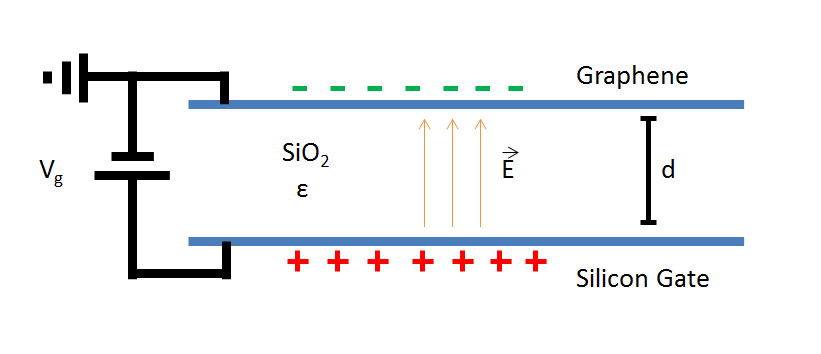
\includegraphics[width=100mm]{GrapheneDevice.png}

Now lets derive the expression for the Fermi level in terms of a backgate voltage (assuming no substrate doping, charge impurities, etc..).  The electric field in the parallel plate capacitor set up is $\vec{E} \approx V_G/d$.  However, by Gauss's Law $\oint \vec{E} \cdot d\vec{A} = Q/\epsilon$
\begin{equation}
\vec{E}=\frac{\sigma}{\epsilon}=\frac{e k_F^2}{\epsilon \pi}=\frac{e E_F^2}{\epsilon \pi (\hbar v_F)^2}
\end{equation}
Setting this equal to $V_G/d$, and solving for $E_F$
\begin{equation}
E_F=\sqrt{\frac{\epsilon \pi (\hbar v_F)^2}{e d} V_G}=\hbar v_F \sqrt{\frac{\pi C}{eA} V_G}
\end{equation}
where $C=\epsilon A/d$ is the geometric parallel plate capacitance (I've neglected quantum capacitance in the $\vec{E} \approx V_G/d$ approximation).

\end{document}